% Extension 2: CP-Decomposition Slides

\begin{frame}{Extension 2: Background and Purpose}
    \textbf{CP-Decomposition:} Architectural constraint shifting from \textbf{post-hoc} to \textbf{intrinsic} interpretability
    
    \vspace{0.3cm}
    \textbf{What it replaces:}
    \begin{itemize}
        \item Original: Bilinear layer computes interaction tensor from $W_l$ and $W_r$ matrices
        \item CP: Replaces the bilinear layer structure, directly parameterizing the interaction tensor with rank-$R$ constraint: $W_{cij} = \sum_{r=1}^{R} \lambda_r A_{cr} B_{ir} C_{jr}$
    \end{itemize}
    
    \vspace{0.3cm}
    \textbf{Maintains interpretability:}
    \begin{itemize}
        \item CP factors can still be eigendecomposed
        \item Factors are \textbf{discrete parts} and \textbf{localized} (e.g., top loops, vertical strokes)
        \item More disentangled than dense eigenvectors
    \end{itemize}
    
    \vspace{0.3cm}
    \textbf{Addresses orthogonality limitations:}
    \begin{itemize}
        \item Standard eigendecomposition enforces orthogonality $\to$ entangled features
        \item CP does \textbf{not} enforce orthogonality $\to$ factors naturally overlap
        \item It's efficient: reduces parameters from $\mathcal{O}(d_{\text{hidden}} \times d_{\text{in}}^2)$ to $\mathcal{O}(R \times d_{\text{in}})$
    \end{itemize}
    
    \vspace{0.2cm}
    \small
    Three variants: Fixed CP, Lambda CP (L1), Gated CP (L0)
\end{frame}

\begin{frame}{Extension 2: Results - It Works!}
    \begin{columns}
        \column{0.5\textwidth}
        \textbf{Accuracy vs Rank Tradeoff:}
        \begin{itemize}
            \item Accuracy increases with rank
            \item At $R=256$: \textbf{93.8\%} accuracy
            \item Effective rank: \textbf{17.5}
        \end{itemize}
        
        \vspace{0.3cm}
        \textbf{Comparison:}
        \begin{itemize}
            \item Original (dense): 97.5\%
            \item CP ($R=256$): 93.8\%
            \item Drop: 3.7 pp
        \end{itemize}
        
        \vspace{0.3cm}
        \textbf{But:} Drastic runtime improvement!
        
        \column{0.5\textwidth}
        \begin{figure}
            \centering
            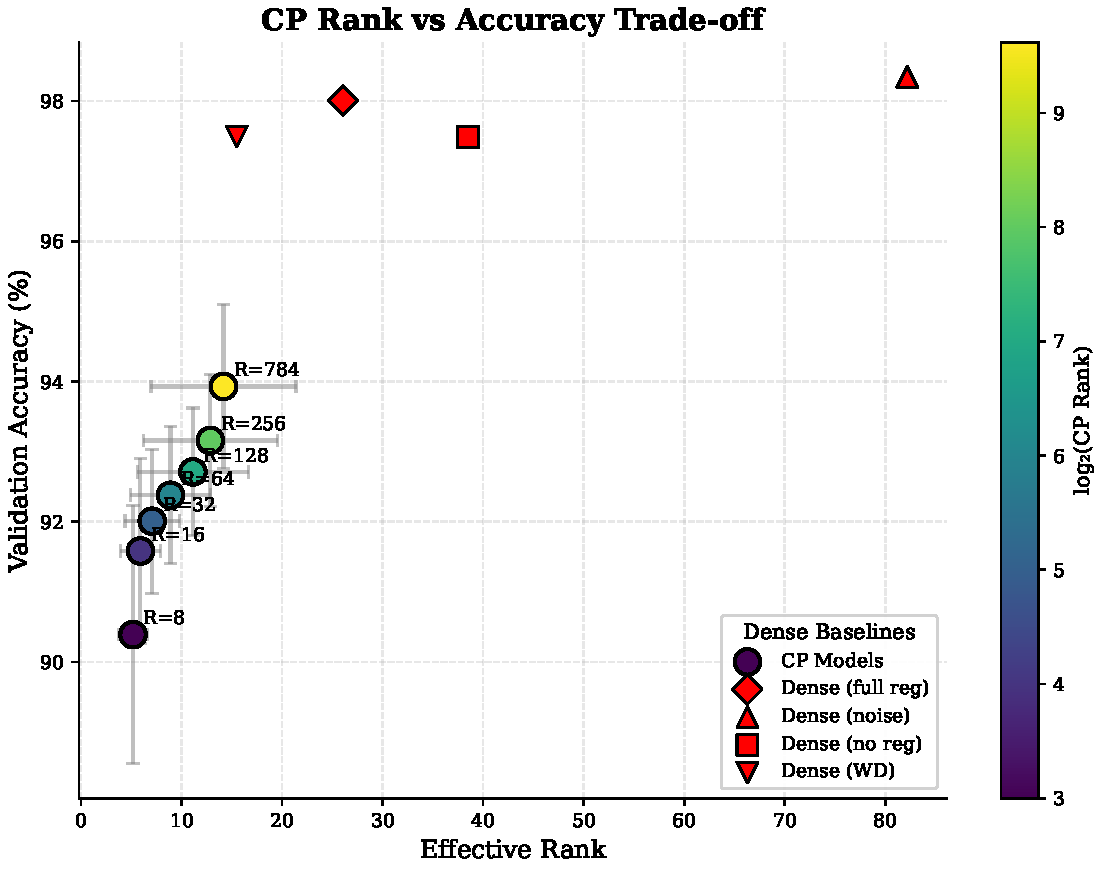
\includegraphics[width=\textwidth]{../Report/figures/extension_cp/cp_rank_accuracy_tradeoff.pdf}
            \caption{Accuracy vs Rank Tradeoff}
        \end{figure}
    \end{columns}
\end{frame}


\begin{frame}{Extension 2: Key Figures}
    \begin{columns}
        \column{0.5\textwidth}
        \begin{figure}
            \centering
            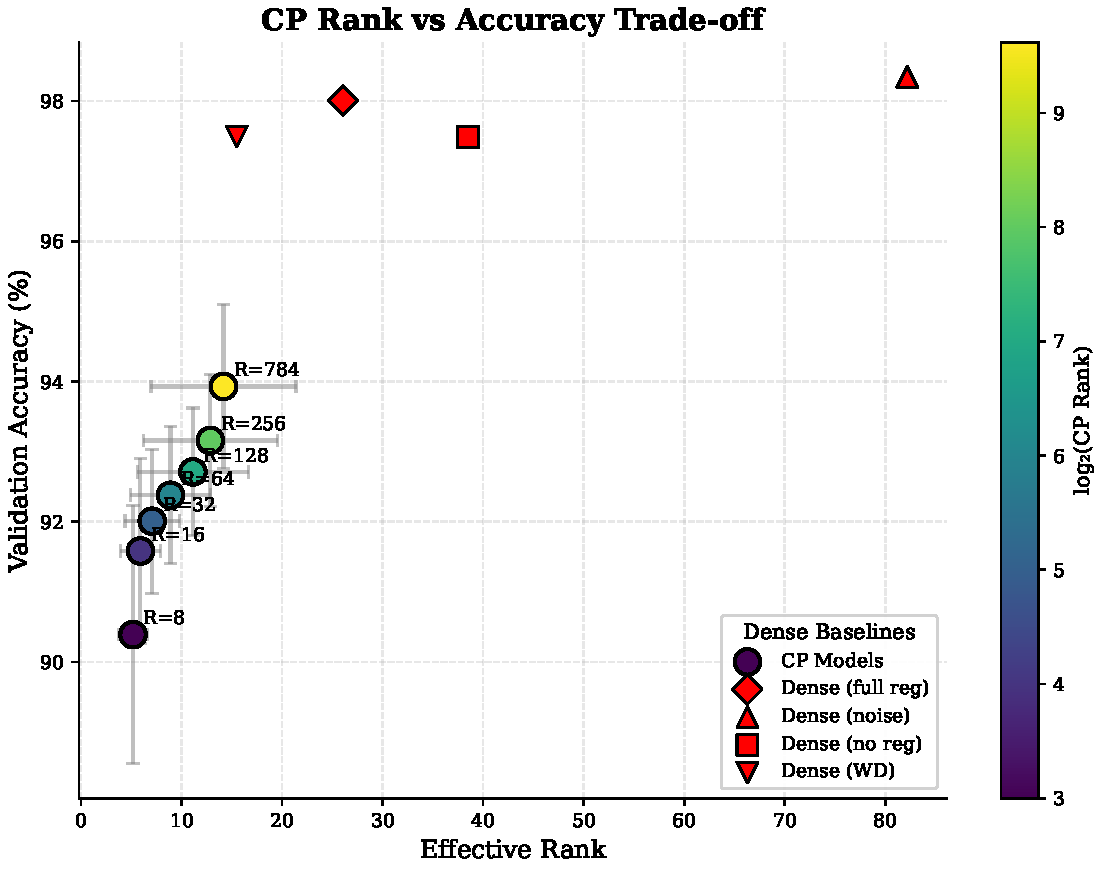
\includegraphics[width=\textwidth]{../Report/figures/extension_cp/cp_rank_accuracy_tradeoff.pdf}
            \caption{Accuracy vs Rank Tradeoff}
        \end{figure}
        
        \column{0.5\textwidth}
        \begin{table}[h]
            \centering
            \small
            \begin{tabular}{lcccc}
                \toprule
                Experiment & Runs & Wall (h) & GPU-h & CO2 (kg) \\
                \midrule
                Vision (Section 4)$^\dagger$ & 81 & 1.22 & 1.11 & 0.039 \\
                Language (Section 5)$^\ddagger$ & 2 & 0.19 & 0.07 & 0.005 \\
                Extension 1 & 15 & 0.58 & 0.58 & 0.020 \\
                Extension 2 (CP) & 105 & 0.05 & 0.05 & 0.004 \\
                \midrule
                \textbf{Total} & \textbf{203} & \textbf{2.04} & \textbf{1.81} & \textbf{0.067} \\
                \bottomrule
            \end{tabular}
            \caption{Environmental impact (CO2 via \texttt{codecarbon})}
        \end{table}
        \footnotesize
        $^\dagger$Some experiments on local M4\\
        $^\ddagger$Language experiments on local M4 (MPS)
    \end{columns}
\end{frame}

\begin{frame}{Extension 2: Disentangled Factors}
    \begin{center}
        \begin{figure}
            \centering
            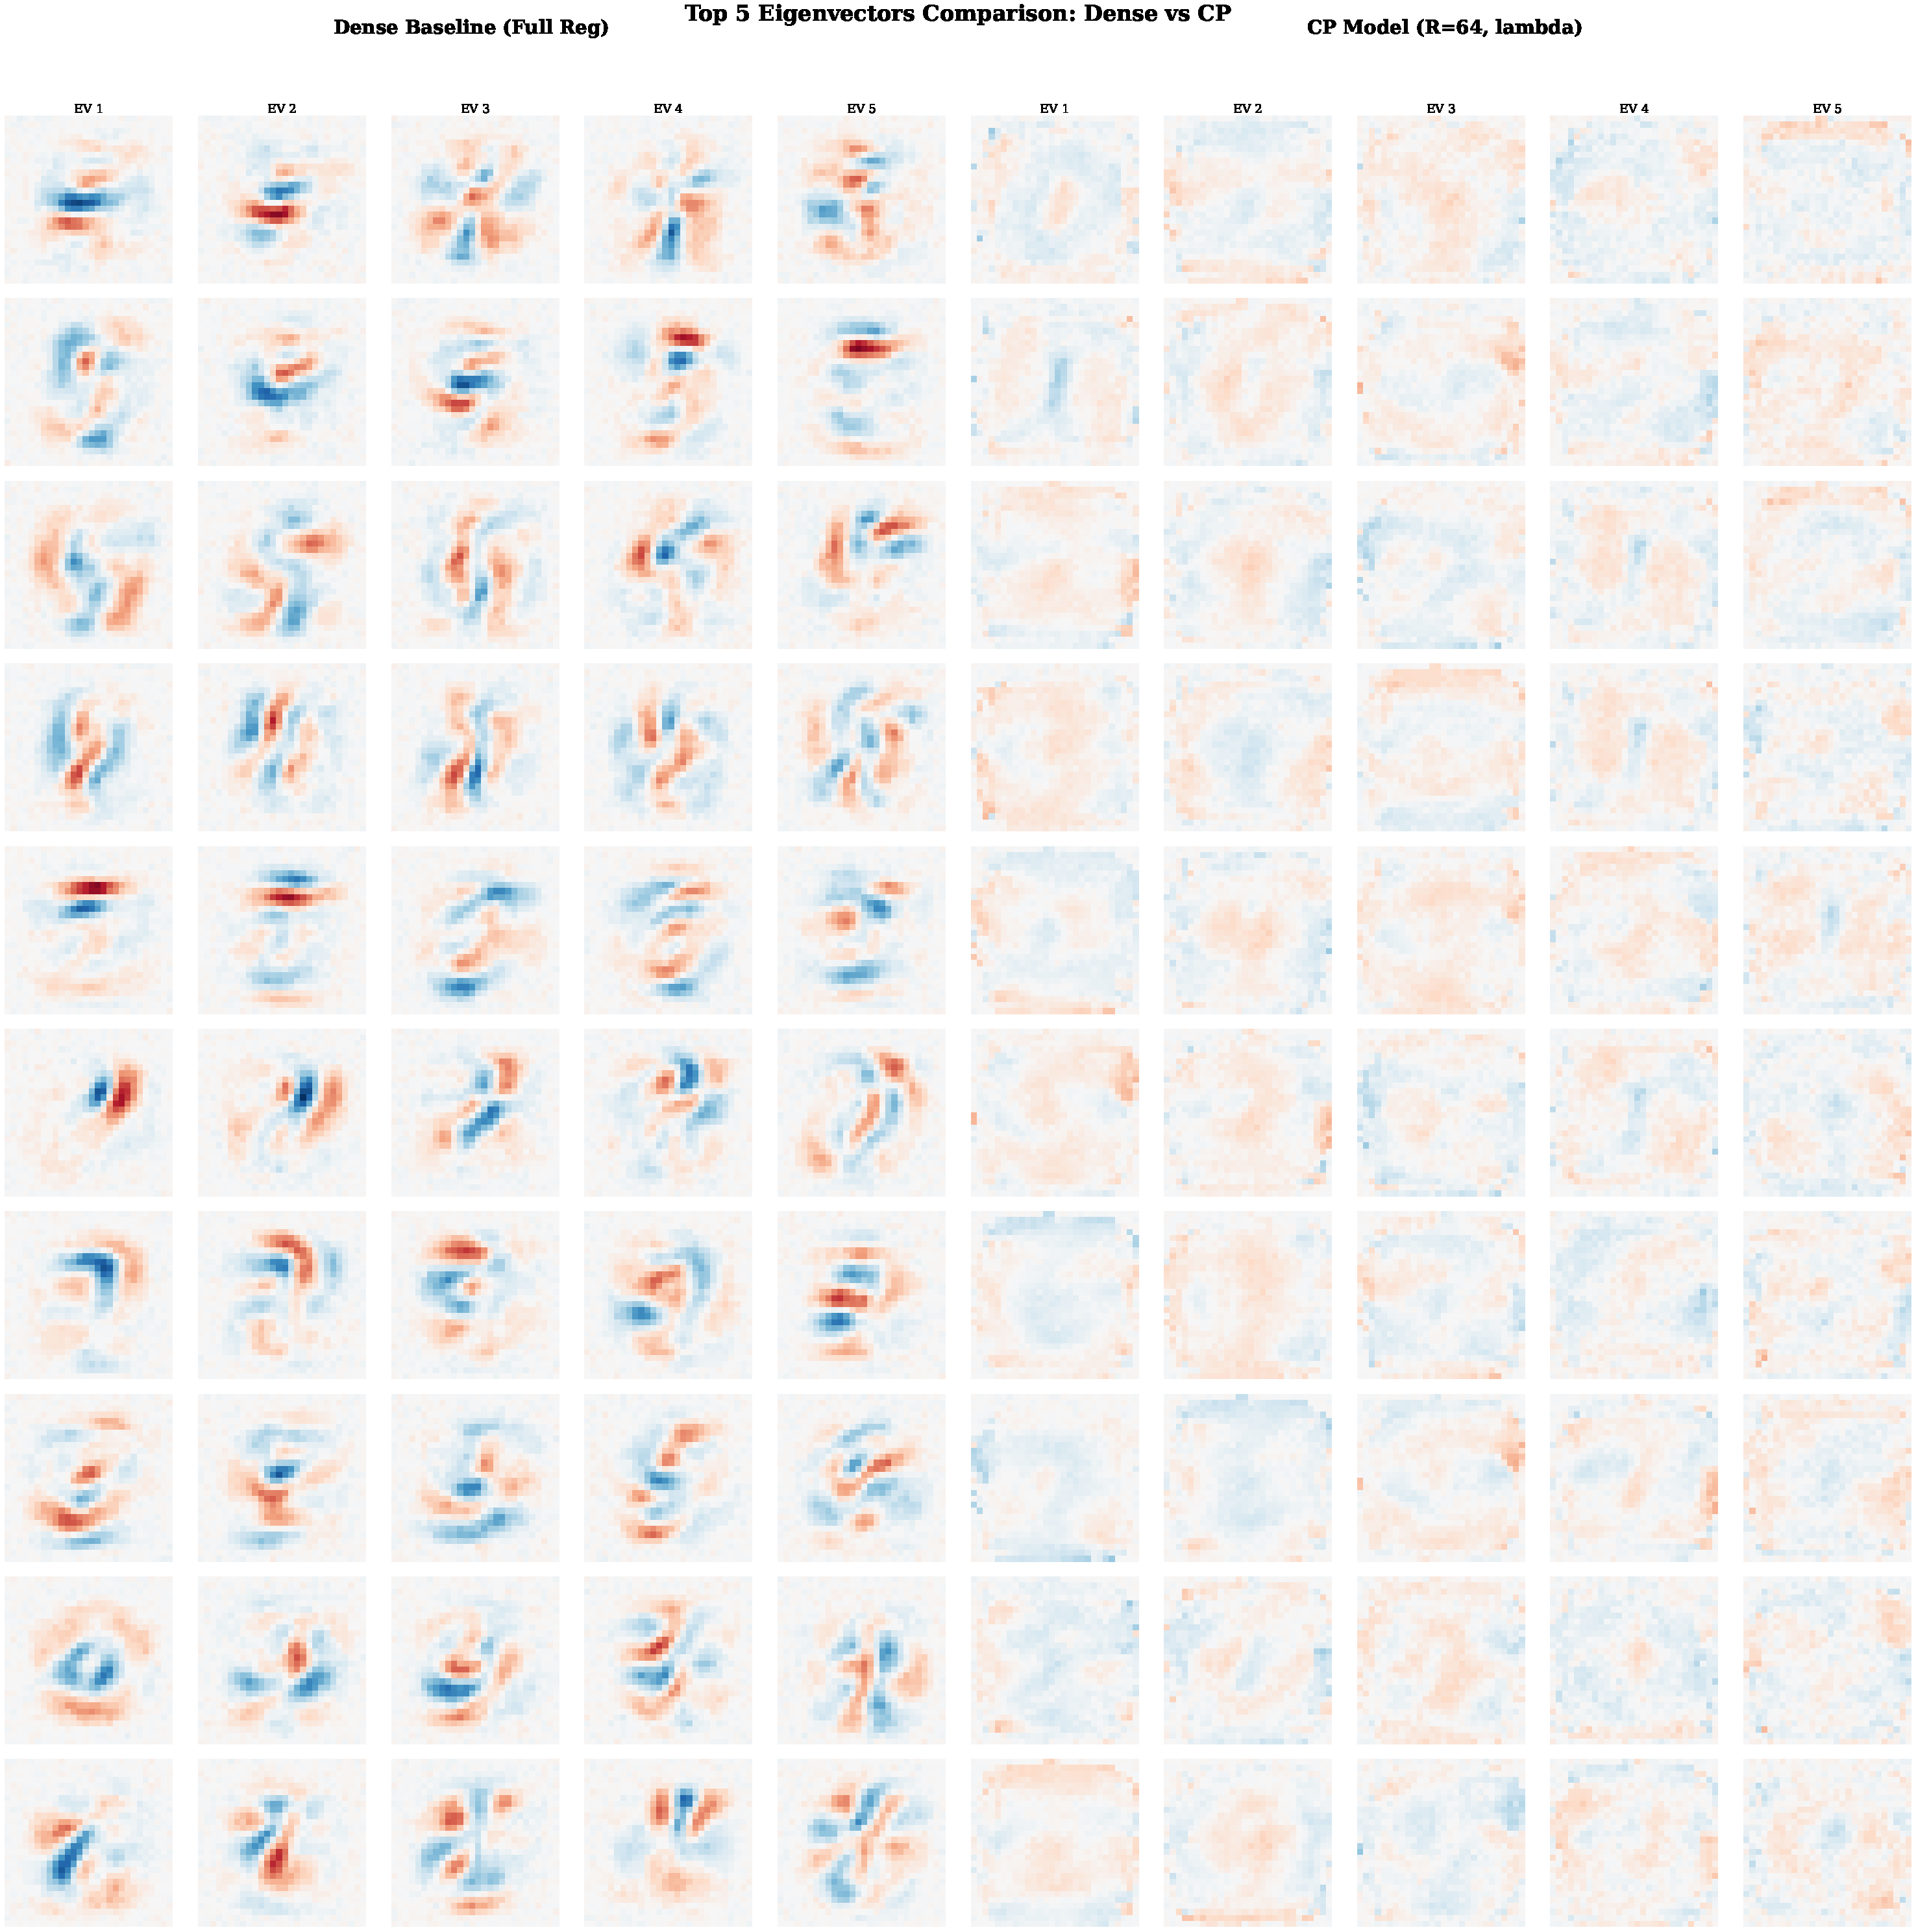
\includegraphics[width=0.8\textwidth]{../Report/figures/extension_cp/cp_top5_eigenvectors_comparison.pdf}
            \caption{Disentangled Factors}
        \end{figure}
        \vspace{0.3cm}
        \small
        CP factors are more \textbf{discrete parts} and \textbf{localized} compared to dense eigenvectors
    \end{center}
\end{frame}

\begin{frame}{Conclusion}
    \textbf{Main Contributions:}
    \begin{itemize}
        \item \textbf{Vision:} Fully reproduced
        \begin{itemize}
            \item Effective rank ratio 0.40 $<$ 0.5 \checkmark
            \item Interpretable eigenvectors confirmed
        \end{itemize}
        
        \item \textbf{Language:} Placeholder (to be filled)
        
        \item \textbf{Extension 1:} Cross-dataset robustness
        \begin{itemize}
            \item Generalization works! (97.7\% cross-dataset accuracy)
            \item Quadratic Form Similarity successfully discriminates
        \end{itemize}
        
        \item \textbf{Extension 2:} CP-decomposition
        \begin{itemize}
            \item 93.8\% accuracy at $R=256$ with drastic runtime improvement
            \item Disentangled, atomic feature representations
        \end{itemize}
    \end{itemize}
\end{frame}
